\documentclass[12pt]{article}
\usepackage[dvips]{epsfig}
\usepackage{url}
\usepackage[colorlinks=true]{hyperref}

\begin{document}

\section*{GENESIS: Documentation}

{\bf Related:}
% start: userdocs-tag-replace-items related-do-nothing
% end: userdocs-tag-replace-items related-do-nothing

\section*{The GENESIS Publication System}

A powerful feature of the GENESIS software system is the capacity to track the life cycle of a research project, from creation through development and extension to publication.

\subsection*{Introduction}

The following figure illustrates the global workflows and dataflows that support the GENESIS publication system.

\begin{figure}[h]
  \centering
   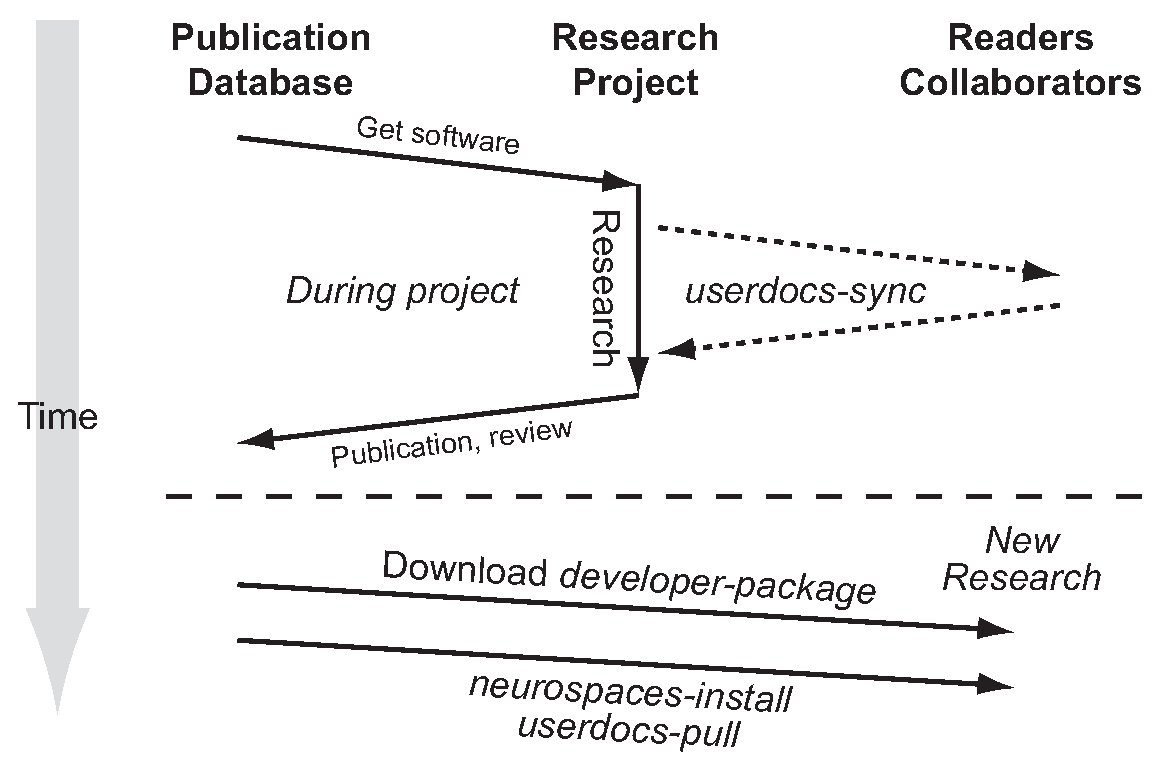
\includegraphics[scale=0.6]{figures/global-workdata-flow.eps}
%\caption{{\bf A Dummy Figure:} Example of \LaTeX\,\,\,code to incorporate a figure into documentation.}
  \label{fig:wf-1}
\end{figure}

\subsection*{Classes of Publication}

The following classes of publication are currently recognized within the GENESIS software platform and have individual workflows to support the publication workflow illustrated above.

\begin{enumerate}
   \item {\bf Document Publication:}
   \item {\bf Tutorial Publication:}
   \item {\bf Model Publication:} A model publication is the publication of a family of mathematical models and their interpretation, usually as annotations to the family of mathematical models. The mathematical models can be run using a simulator where annotations explain their functional components, their relationships, data outputs, and analysis. A model publication can in turn be converted to a tutorial publication.
   \item{\bf Project Publication:} This is the most general class of publication. The G3 \href{../workflow-user/workflow-user.tex}{\bf User Workflow} defines iterators that close the loop between the steps of the user workflow to deliver a GENESIS project. A GENESIS project can be defined as  a model publication but the reverse is not necessarily true. For example, a project publication can be a publication about data mining of the publication database.
\end{enumerate}

\subsection*{Annotation}

There are two classes of annotation that are iterative in the sense that a process may be repeated many times:

\begin{enumerate}
   \item {\bf Automated Annotations:} Automated model interpretation is the same as simulating and running a model to generate results so the results are the first line of annotations.
   \item {\bf Manual Annotations:} Analysis of results.
\end{enumerate}

\end{document}